\begin{frame}
\frametitle{Famous Composers}
\begin{center}
\rowcolors{1}{RoyalBlue!20}{RoyalBlue!5}
\begin{tabular}{|l|c|}\hline
J.\ S.\ Bach & 1685--1750 \\
W.\ A.\ Mozart & 1756--1791 \\
L.\ Beethoven & 1770--1827 \\
F.\ Chopin & 1810--1849 \\
R.\ Schumann & 1810--1856 \\
B.\ Bart\'{o}k & 1881--1945 \\ \hline
\end{tabular}
\end{center}
\end{frame}

\begin{frame}
\frametitle{Two Column Output}
\begin{columns}[c]
\column{1.5in}
Practical \TeX\ 2005\\
Practical \TeX\ 2005\\
Practical \TeX\ 2005
\column{1.5in}
\framebox{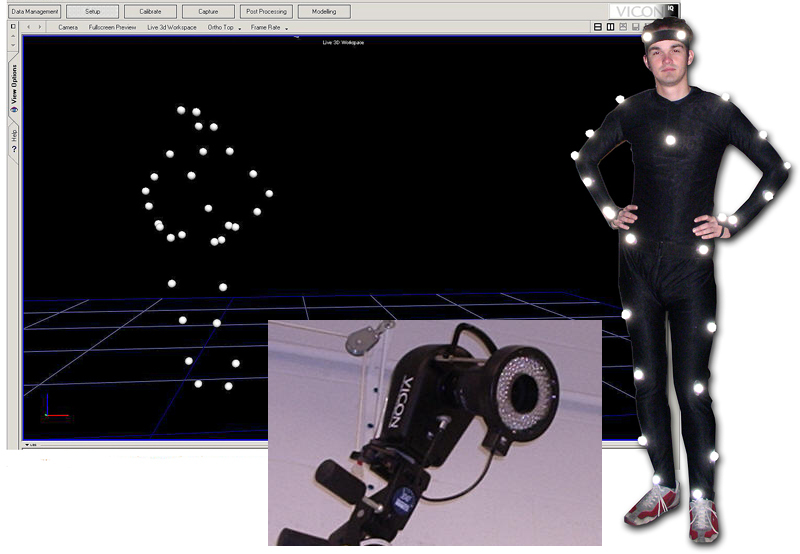
\includegraphics[width=1.5in]{imgs/viconMotionCapture.jpg}}
\end{columns}
\end{frame}

\begin{frame}
\frametitle{Overlays with {\tt pause}}
\setbeamercovered{dynamic}
Practical \TeX\ 2005\\ \pause
Practical \TeX\ 2005\\ \pause
Practical \TeX\ 2005
\end{frame}

\begin{frame}
\frametitle{Tic-Tac-Toe via {\tt tabular}}
\setbeamercovered{invisible}
{\Huge
\begin{center}
\begin{tabular}{c|c|c}
\onslide<9->{O} & \onslide<8->{X} & \onslide<2->{X} \\ \hline
\onslide<6->{X} & \onslide<3->{O} & \onslide<5->{O} \\ \hline
\onslide<10->{X} & \onslide<7->{O} & \onslide<4->{X}
\end{tabular}
\end{center}
}
\end{frame}


\begin{frame}
\frametitle{Tic-Tac-Toe via Graphics Files}
\setbeamercovered{invisible}
\begin{center}
\multiinclude[format=pdf,width=3in]{imgs/hmm}
\end{center}
\end{frame}